\documentclass[11pt]{beamer}
\usepackage[utf8]{inputenc}
\usepackage[T1]{fontenc}
\usepackage[english,french]{babel}
\usepackage{amsfonts,amsmath,amssymb}
\usepackage{tikz,xcolor}
\usepackage[noend]{algpseudocode}
\usepackage{algorithm}
\usepackage{algorithmicx}
\usepackage{stmaryrd}
\usepackage{multicol}
\usetheme{Antibes}
\usecolortheme{whale}
\usetikzlibrary{positioning}

\setbeamertemplate{footline}
{%
  \begin{beamercolorbox}[colsep=1.5pt]{upper separation line foot}
  \end{beamercolorbox}
  \hbox{%
    \begin{beamercolorbox}[wd=0.333333\paperwidth, ht=2.5ex, dp=1.125ex, center]{title in head/foot}%
      \usebeamerfont{author in head/foot}\insertshortauthor%~~\beamer@ifempty{\insertshortinstitute}{}{(\insertshortinstitute)}
    \end{beamercolorbox}%
    \begin{beamercolorbox}[wd=0.333333\paperwidth, ht=2.5ex, dp=1.125ex, center]{title in head/foot}%
      \usebeamerfont{title in head/foot}\insertshorttitle
    \end{beamercolorbox}%
    \begin{beamercolorbox}[wd=0.333333\paperwidth, ht=2.5ex, dp=1.125ex, center]{title in head/foot}%
      \usebeamerfont{title in head/foot}\insertframenumber/\inserttotalframenumber\hspace*{2ex}
    \end{beamercolorbox}}
  \begin{beamercolorbox}[colsep=1.5pt]{lower separation line foot}
  \end{beamercolorbox}
}
%\AtBeginSection[]
%{
%	\begin{frame}
%	\frametitle{Content} 
%	\tableofcontents[currentsection,hideothersubsections]
%	\end{frame}
%}


\title{SPOT : Sliced Partial Optimal Transport}
\author{Quentin \bsc{Spinat}}
\date{}

\begin{document}

\begin{frame}
\titlepage
\end{frame}
	
\section*{Introduction}	

\subsection*{Goal}
	
\begin{frame}
We want to find the optimal injective assignment $a : \llbracket 1;m \rrbracket \rightarrow \llbracket 1;n \rrbracket$ between two point sets $X$ and $Y$ of different sizes $m\leqslant n$.

\begin{figure}[H]
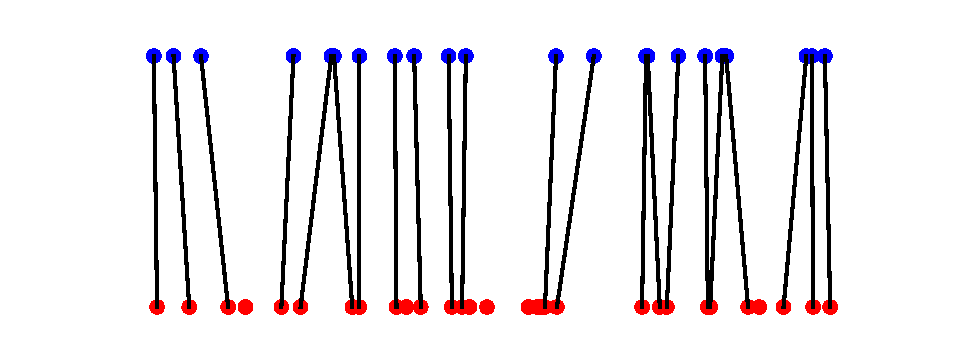
\includegraphics[scale = 0.5]{a_fig.pdf}
\caption{Partial Optimal Assignment in 1D}\label{a_fig}
\end{figure}

\end{frame}

\subsection*{Method}

\begin{frame}

\begin{itemize}
\item Efficient 1D injective assignment algorithm
\item Sliced optimal transport 
\item Combined with other methods if needed (Iterative Closest Point,...)
\end{itemize}

\end{frame}

\subsection*{Applications}

\begin{frame}

\begin{itemize}
\item Color Transfer for images with content in different proportion
\end{itemize}

\begin{figure}[H]
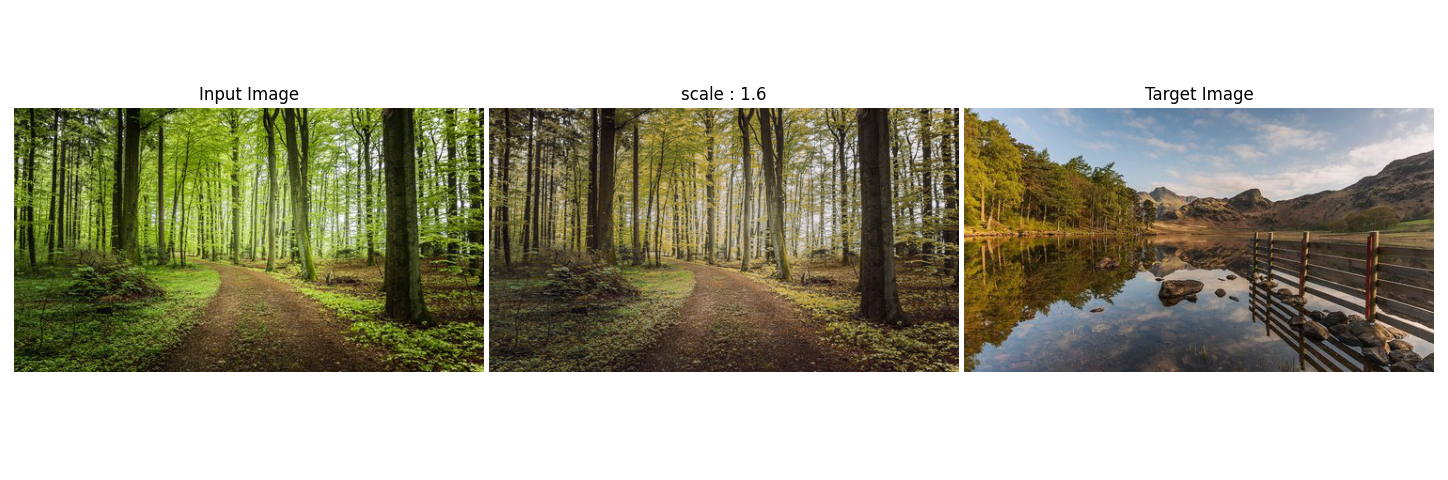
\includegraphics[scale = 0.3,trim= 0cm 2.5cm 0cm 2.5cm]{exemple_image.png}
\caption{Color Transfer}\label{ex_im}
\end{figure}

\end{frame}

\begin{frame}

\begin{itemize}
\item Point cloud registration for point clouds of different sizes
\end{itemize}

\begin{figure}[H]
\centering
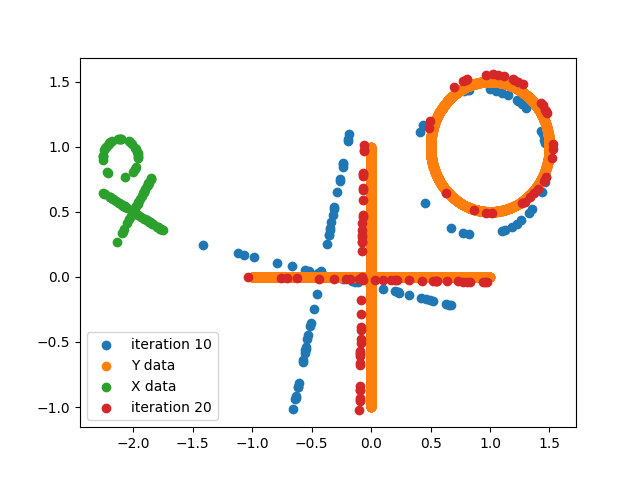
\includegraphics[scale = 0.35]{circle_cross_shape2.png}
\caption{Point cloud Registration}\label{ex_shape}
\end{figure}

\end{frame}

%\begin{frame}
%Slide 2
%\begin{block}{Définition}
%Définition
%\end{block}
%\end{frame}

\subsection*{Content}	
	
\begin{frame}
\tableofcontents[]
\end{frame}

\section{Partial Transport in 1-D}

\subsection{Nearest Neighbor Assignment}

\begin{frame}

\frametitle{Partial Transport in 1-D}

The core of the method relies on the {\color{red}nearest neighbor assignment} $t$, which is easy to compute : the algorithm consists in {\color{red} scanning $X$ and $Y$ simultaneously from left to right} and comparing their value.

\begin{algorithm}[H]
\scriptsize
\caption{Nearest Neighbor Assignment}\label{t}
\begin{multicols}{2}
\hspace*{\algorithmicindent} \textbf{Input:} sorted $X,Y$\\
\hspace*{\algorithmicindent} \textbf{Output:} $t$ 
\begin{algorithmic}[2]
\State $i\gets 1$
\State $j\gets 1$
\While{$i<m$}
	\If{$x_i \leqslant y_j$}
		\State $t[i] \gets j$
		\State $i \gets i+1$
    \ElsIf {$j=n$}:
        \State $t[i] \gets n$
        \State $i \gets i+1$
    \ElsIf {$y_{j+1}<x_i$}
        \State $j \gets j+1$
    \ElsIf {$|x_i-y_j|<|x_i-y_{j+1}|$}:
        \State $t[i] \gets j$
        \State $i \gets i+1$
    \Else
        \State $t[i] \gets j+1$
        \State $j \gets j+1$
        \State $i \gets i+1$
    \EndIf
\EndWhile
\State \Return{$t$}
\end{algorithmic}
\end{multicols}
\end{algorithm}

\end{frame}

\begin{frame}
\begin{figure}[H]
\centering
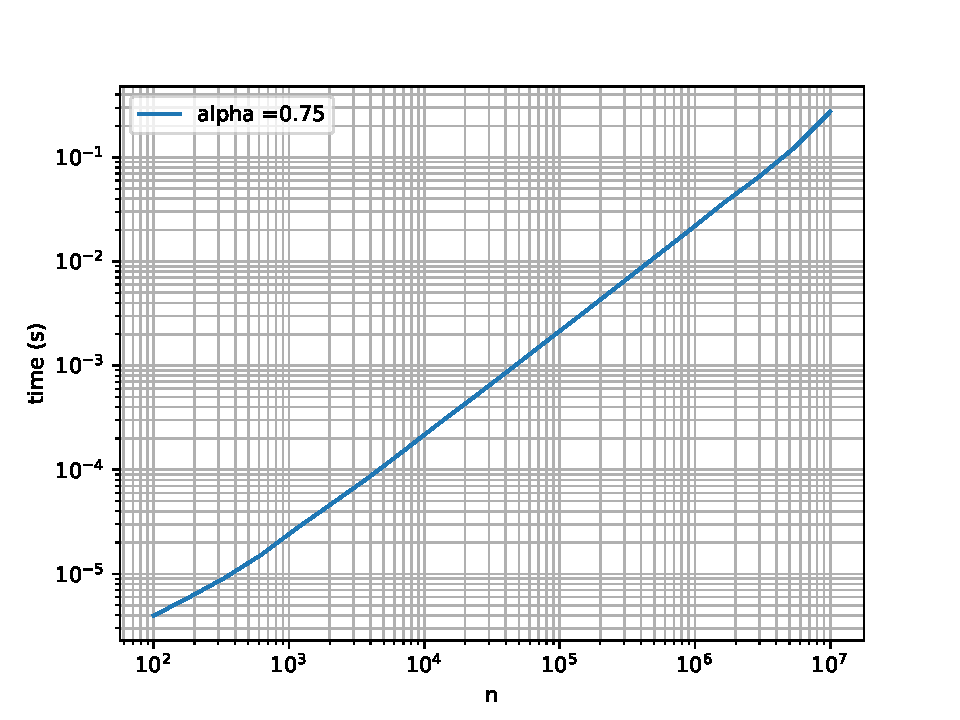
\includegraphics[scale=0.48]{t_time.pdf}
\caption{Mean time over $100$ simulations for Nearest Neighbor Assignment with respect to $n$, $\alpha=\dfrac{m}{b}=0.75$, logscale}\label{t_time}
\end{figure}
\end{frame}

\subsection{Quadratic Time Algorithm}

\begin{frame}

Nearest Neighbor assignment $t$ is {\color{red}not injective} 
\begin{itemize}
\item We need to resolve issues where $t[i]=t[j]$
\end{itemize} 
Method : 
\begin{itemize}
\item Find $a_{m'}$ optimal injective assignment between $X' = \{x_i \}_{i \in \llbracket 1;m' \rrbracket} $ and $Y$ thanks to $t$ and $a_{m'-1}$, progressively increasing $m'$ from $1$ to $m$. 
\end{itemize}

\begin{figure}
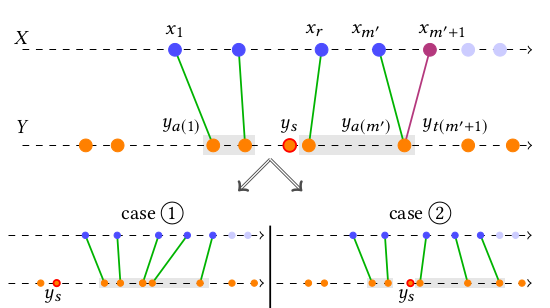
\includegraphics[scale=0.4]{quad_cases.png}
\end{figure}

\end{frame}

\begin{frame}

\begin{algorithm}[H]
\caption{Quadratic Partial Optimal Assignment}\label{a_quad}
\begin{multicols}{2}
\scriptsize
\hspace*{\algorithmicindent} \textbf{Input:} sorted $X,Y$\\
\hspace*{\algorithmicindent} \textbf{Output:} $a$ 
\begin{algorithmic}[2]
\State compute $t$
\State $a[1] \gets t[1]$
\For{$i$ from $1$ to $m-1$}
	\If{$t[i+1] > a[i]$}
		\State $a[i+1] \gets t[i+1]$
		\State update $r$
    \Else
        \State $w_1 \gets \sum_{k=r}^{i} (x_k - y_{a[k]})^2 + (x_{i+1} - y_{a[i]+1})^2$
        \State $w_2 \gets \sum_{k=r}^{i} (x_k - y_{a[k]-1})^2 + (x_{i+1} - y_{a[i]})^2$
        \If {$w_1\leqslant w_2$} \Comment{Case 1}
        	\State $a[i+1] \gets a[i]+1$
        \Else \Comment{Case 2}
        	\State $a[i+1] \gets a[i]$
        	\State $a[r:i] \gets a[r:i]-1$
        	\State update $r$
        \EndIf
    \EndIf
\EndFor
\State \Return{$a$}
\end{algorithmic}
\end{multicols}
\end{algorithm}
\end{frame}

\begin{frame}
\begin{figure}[H]
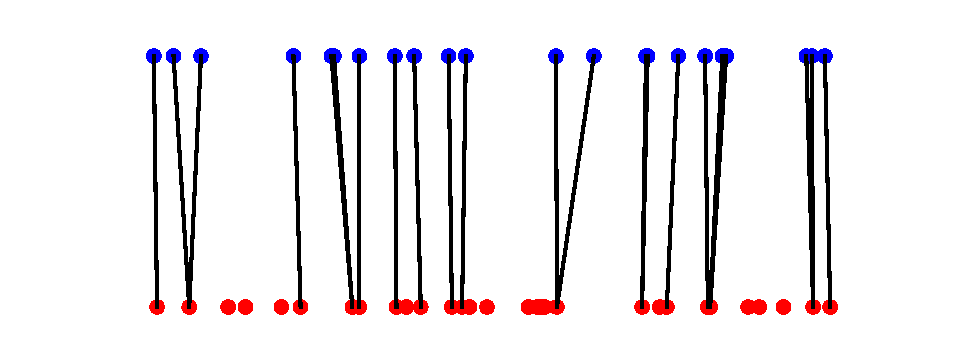
\includegraphics[scale=0.45]{t_fig.pdf}
\caption{Nearest Neighbor Assignment}\label{t_fig}
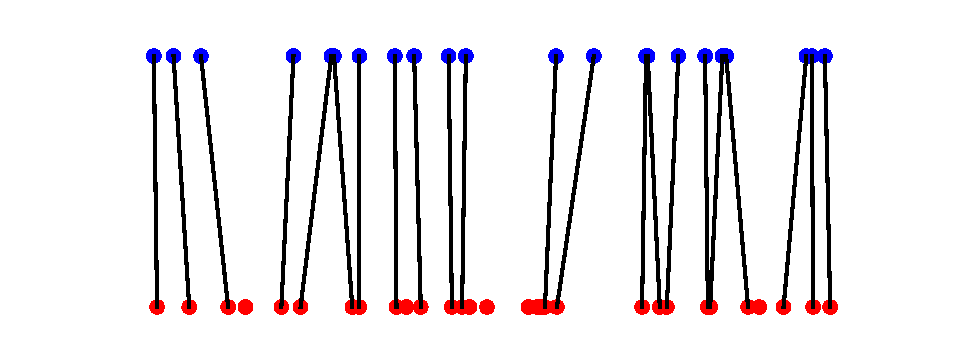
\includegraphics[scale=0.45]{a_fig.pdf}
\caption{Partial Optimal Assignment}\label{a_fig}
\end{figure}
\end{frame}

\begin{frame}
\begin{figure}[H]
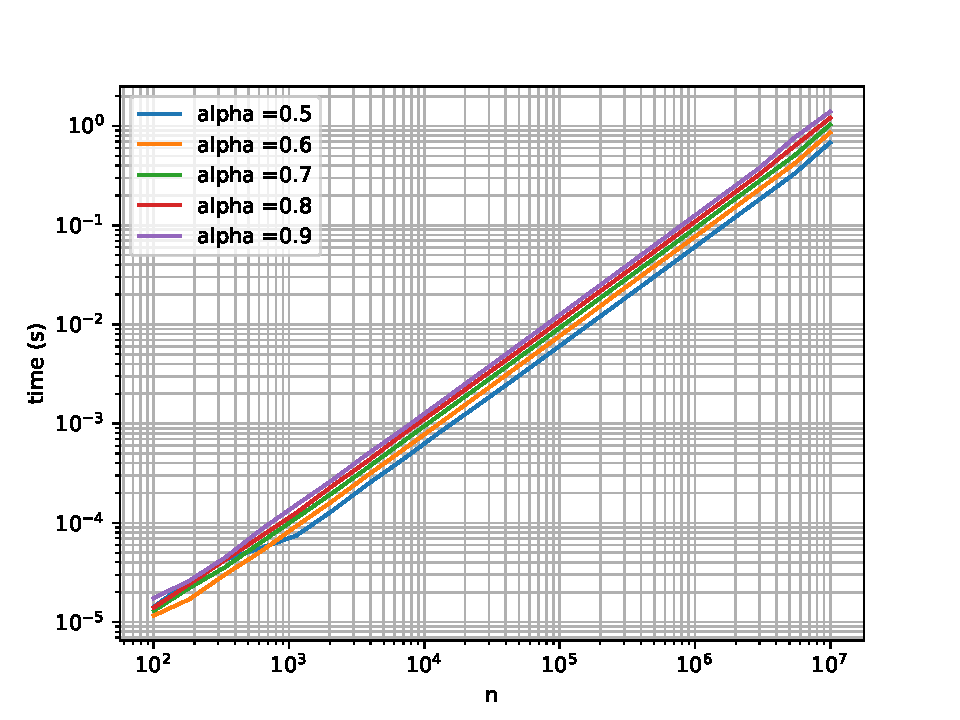
\includegraphics[scale=0.48]{a_time.pdf}
\caption{Mean time over $100$ simulations for Quadratic Partial Optimal Assignment with respect to $n$, for different values of $\alpha=\dfrac{m}{n}$, logscale}\label{a_time}
\end{figure}
\end{frame}

\begin{frame}

There are {\color{red}easy sub-cases} that can accelerate the algorithm:
\begin{itemize}
\item If $m=n$ or $m=n-1$ 
\item If there exists $i$ such that $X[1:i] \leqslant Y[1:i]$
\item If there exists $i$ such that $Y[i:n] \leqslant X[i:m]$
\item If $t$ is injective
\item We can decrease the size of $Y$ according to the number of non-injective values of $t$
\end{itemize}

Finally we don't need to compute $w_1$ and $w_2$ entirely when we choose the case 1
\end{frame}


\subsection{Quasilinear Time Problem Decomposition}

\begin{frame}
Goal : 
\begin{itemize}
\item {\color{red}decompose the original problem into many easier subproblems}, which can be solved {\color{red}independently} (hence in parallel) with the previous partial optimal assignment algorithm.
\end{itemize}

\begin{figure}[H]
\begin{tikzpicture}
\node (bad) {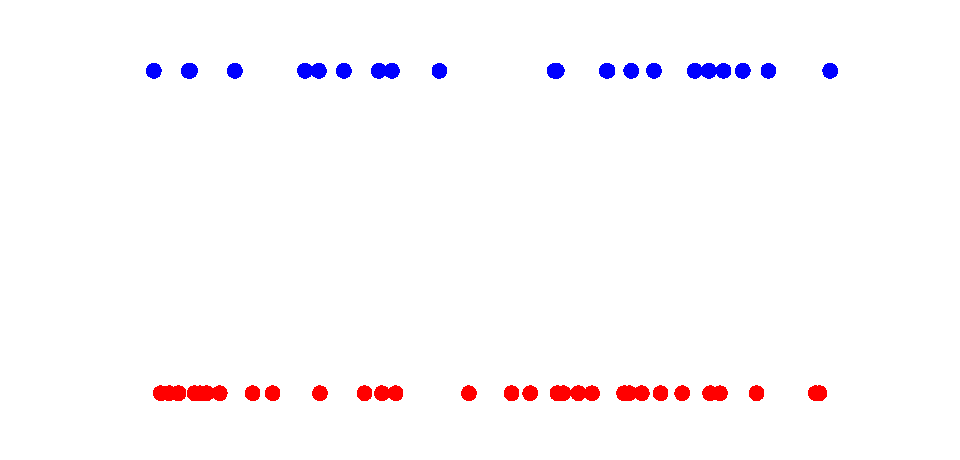
\includegraphics[scale = 0.4,trim = 2cm 1cm 2cm 1cm]{before_decomp.pdf}};
\node (good) [right=of bad] {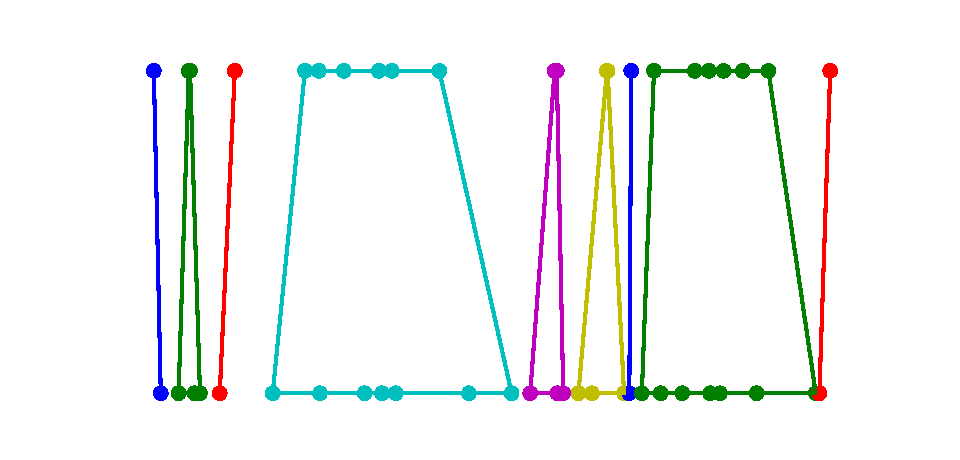
\includegraphics[scale=0.4,trim = 2cm 1cm 2cm 1cm]{decomp_fig.pdf}};

\node (a) [] at (bad.east) {};
\node (b) [] at (good.west) {};

\draw [ultra thick,black,->] (a) to[left] (b);
\end{tikzpicture}
\caption{Assignment problem decomposition}\label{decomp_fig}
\end{figure}

\end{frame}

\begin{frame}

\begin{algorithm}[H]
\caption{Decomposition of the assignment problem}\label{subproblem}
\scriptsize
%\begin{multicols}{2}
\hspace*{\algorithmicindent} \textbf{Input:} sorted $X,Y$\\
\hspace*{\algorithmicindent} \textbf{Output:} $A$ 
\begin{algorithmic}[2]
\State Compute $t$
\For{$m'$ from $1$ to $m$}
	\If{$t[m']$ not considered by any subproblem}
		\State Create new subproblem with $x_{m'}$ and $y_{t[m']}$
    \Else
        \State Consider last subproblem $A_{k'}$
        \If {$t[m'] \neq t[m'-1]$}
        	\State Add $x_{m'}$ to $X_{k'}$ and expand $Y_{k'}$ on the right only
        \Else
        	\While {first point before $Y_{k'}$ is considered by previous subproblem} 
        		\State Merge $A_{k'}$ with previous subproblem
        	\EndWhile
        	\State Add $x_{m'}$ to $X_{k'}$ and expand $Y_{k'}$ on the right and on the left
        \EndIf
    \EndIf
\EndFor
\State \Return{$A$}
\end{algorithmic}
%\end{multicols}
\end{algorithm}

\end{frame}

\begin{frame}
\begin{figure}
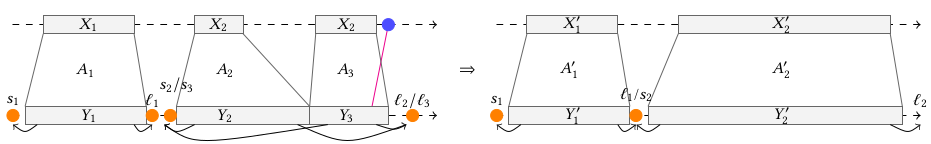
\includegraphics[scale=0.35, trim = 1cm 0cm 0cm 0cm]{ex_decomp.png}
\caption{Problem decomposition : Merging two subproblems to expand on the right and on the left}
\end{figure}
\end{frame}

\begin{frame}
\begin{figure}[H]
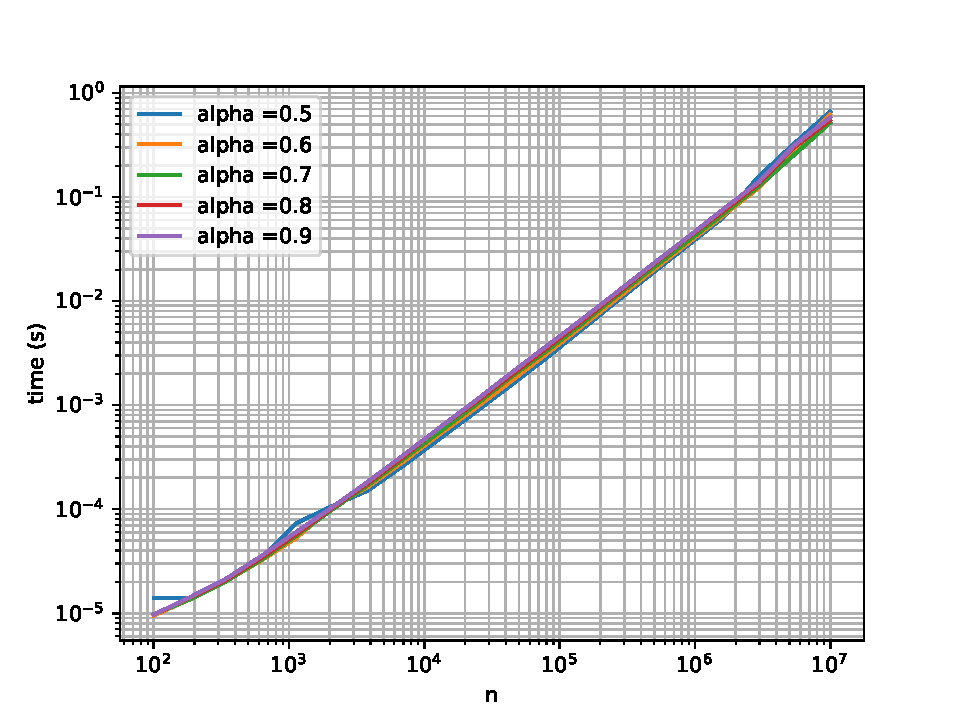
\includegraphics[scale=0.48]{decomp_time.pdf}
\caption{Mean time over $100$ simulations for the decomposition of the assignment problem with respect to $n$, for different values of $\alpha=\dfrac{m}{n}$, logscale}\label{decomp_time}
\end{figure}
\end{frame}


\section{Sliced Partial Transport}

\begin{frame}

\frametitle{Sliced Partial Transport}

Goal :
\begin{itemize}
\item Use 1-D partial optimal transport to solve d-D partial optimal transport
\end{itemize}


Instead of directly solving :
\begin{equation}
\min_{\tilde{X}} W_S(\tilde{X},Y)
\end{equation}

We do the minimization : 
\begin{equation}
\min_{\tilde{X}} \int_{S^{d-1}} W_S(Proj_\omega(\tilde{X}),Proj_\omega(Y))\,d\omega
\end{equation}
\end{frame}

\begin{frame}
We use a {\color{red}stochastic gradient descent}

The gradient of $E_\omega(X_k) = W_S(Proj_\omega(X_k),Proj_\omega(Y))$ is 
\begin{equation}
\nabla_{X}  E_\omega(X_k) = Proj_\omega(X_k)-Proj_\omega(Y \circ a)
\end{equation}

\begin{algorithm}[H]
\caption{Stochastic Gradient Descent}\label{SGD}
\scriptsize
%\begin{multicols}{2}
\hspace*{\algorithmicindent} \textbf{Input:} sorted $X,Y$\\
\hspace*{\algorithmicindent} \textbf{Output:} $X^*$ 
\begin{algorithmic}[2]
\State Initialize $X_0=X$
\For{$k$ from $0$ to $n_{iter}-1$}
	\State Choose $\omega$ random direction
	\State Compute the optimal Partial assignment $a$ between $Proj_\omega(X_k)$ and $Proj_\omega(Y)$
	\State Update $X_{k+1} \gets X_k - \eta_k \nabla_{X}  E_\omega(X_k)$
\EndFor
\State \Return{$X_{n_{iter}}$}
\end{algorithmic}
%\end{multicols}
\end{algorithm}

\end{frame}

\section{Results}

\subsection{Color Transfer}

\begin{frame}
\frametitle{Results : Color Transfer}

Goal :
Transferring the colors of an image to second image.
\bigskip

Slices Partial Optimal Transport can be useful for color transfer {\color{red}between images with their content not in the same proportion}.
\bigskip

A classical color transfer algorithm between an image with a lot of trees and an image with a lot of sky will result in an image where the trees are blue. \\
\bigskip
Idea :
\begin{itemize}
\item {\color{red}Upscale} the target image and use sliced partial optimal transport
\end{itemize}
\end{frame}

\begin{frame}
\begin{figure}
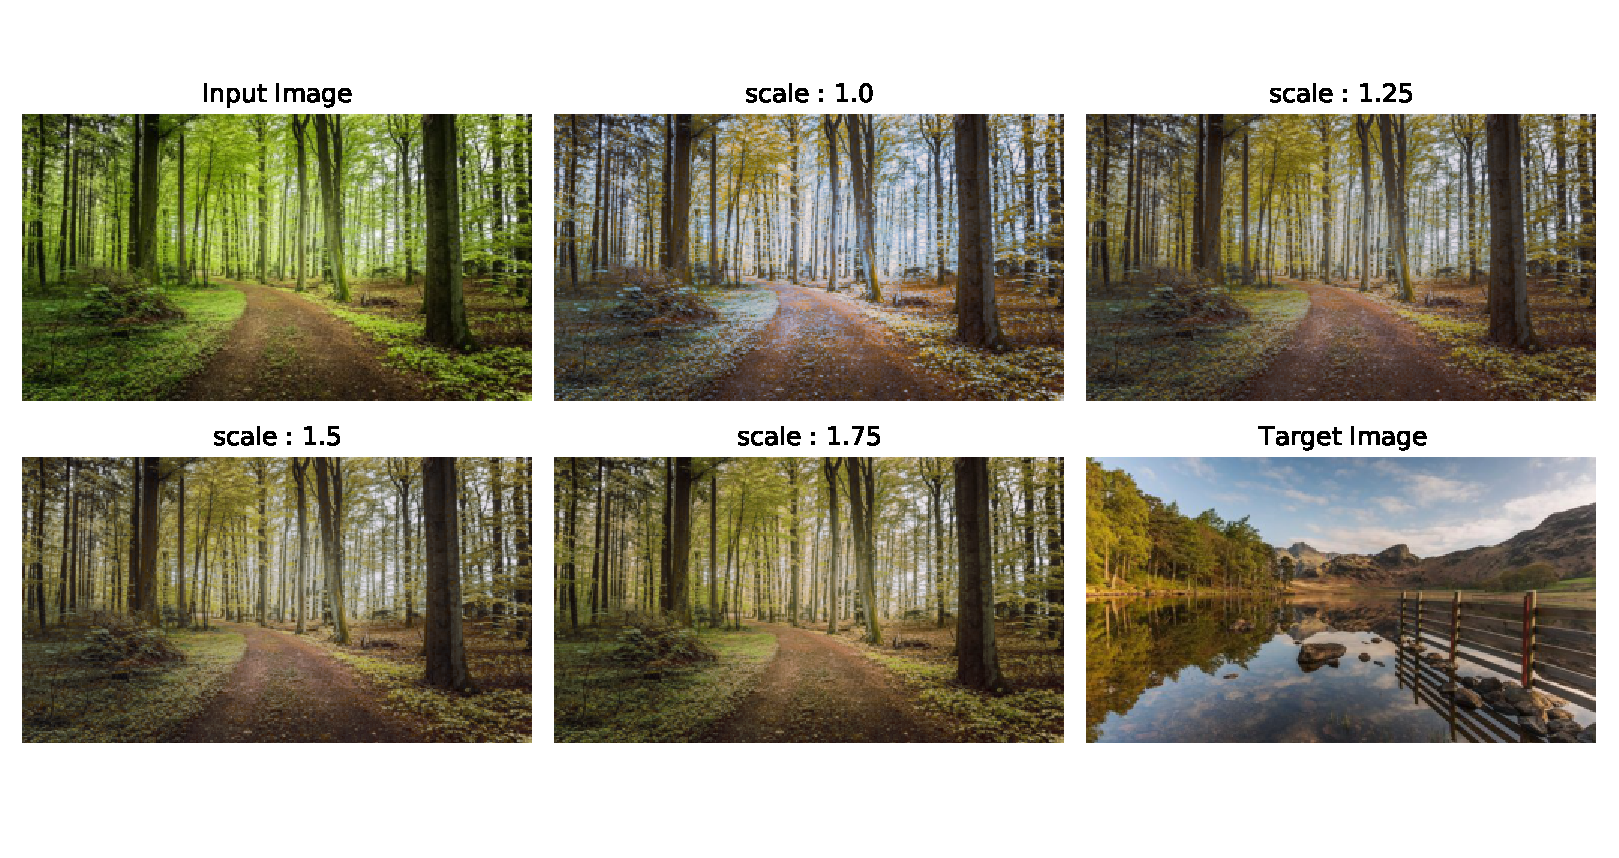
\includegraphics[width = \textwidth]{landscape42_6.pdf} \label{42_fig}
\caption{Color transfer for different upscaling values}
\end{figure}
\end{frame}

%\begin{frame}
%\begin{figure}
%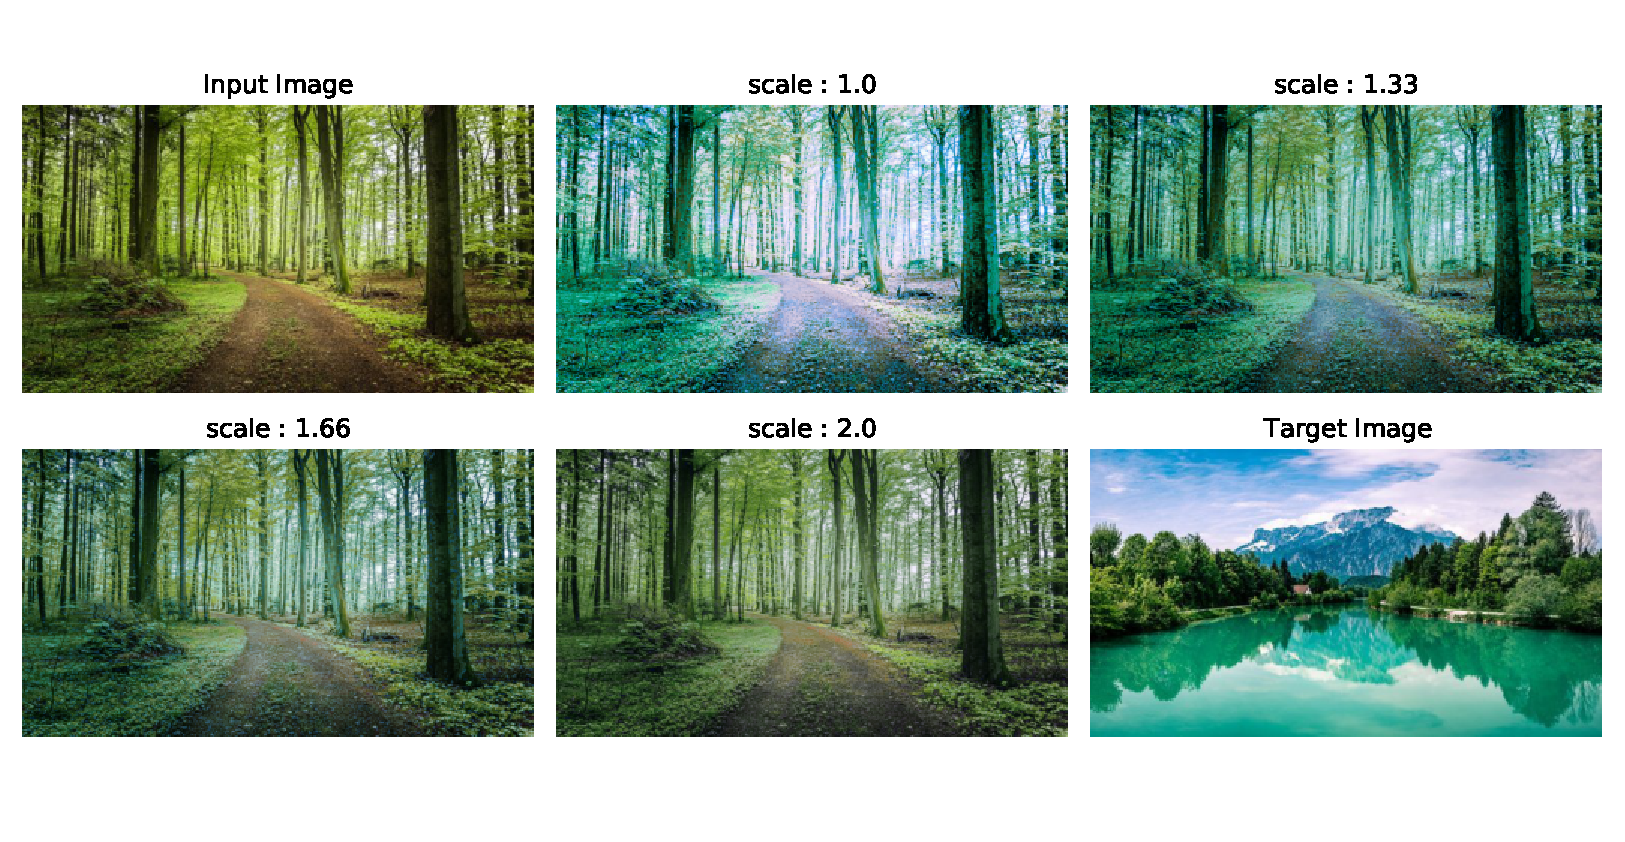
\includegraphics[width = \textwidth]{landscape41_6.pdf} \label{41_fig}
%\caption{Color transfer for different upscaling values}
%\end{figure}
%\end{frame}

\begin{frame}
\begin{figure}
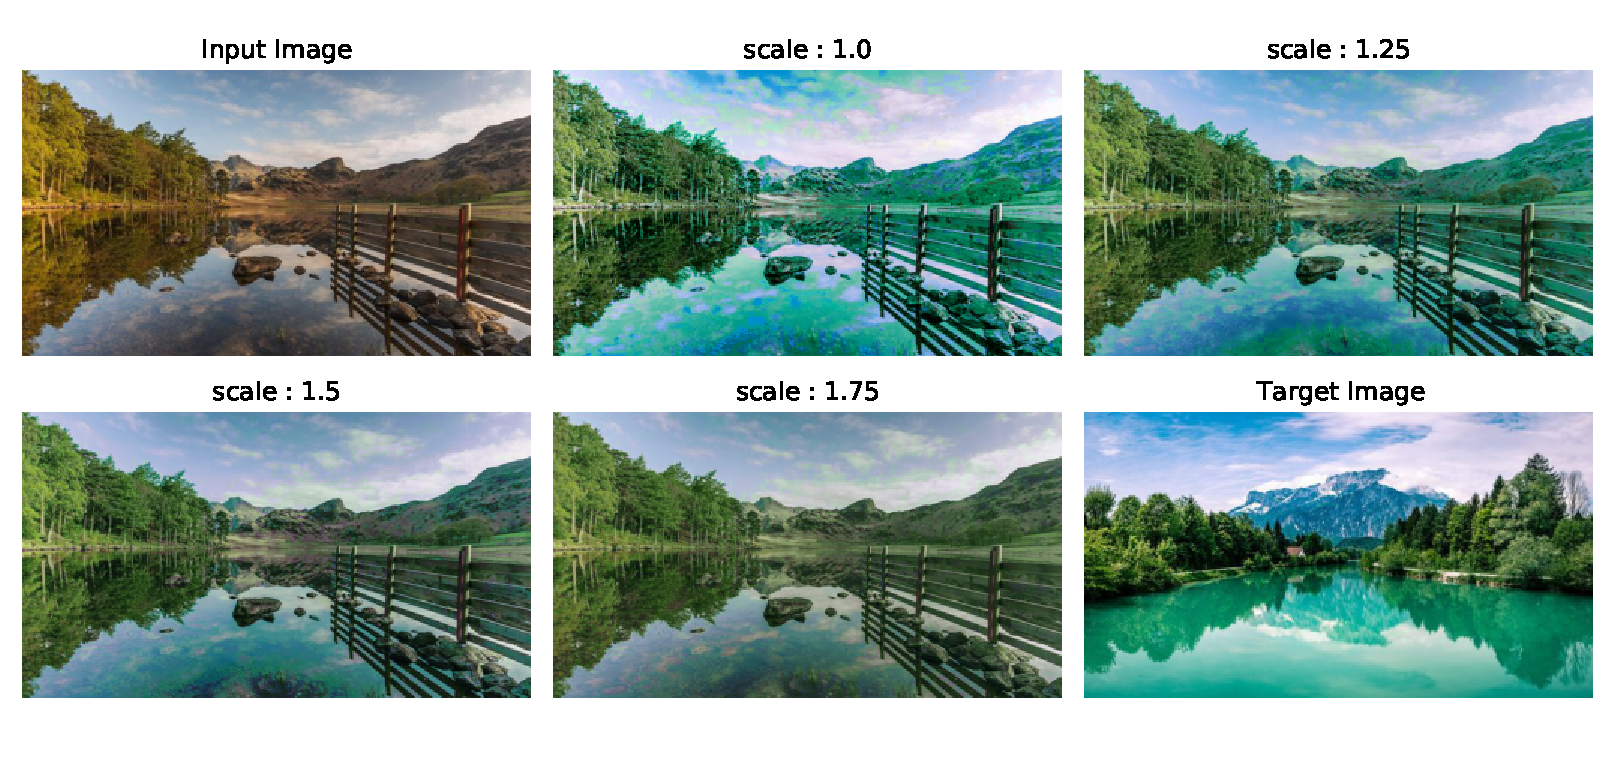
\includegraphics[width = \textwidth]{landscape21_6.pdf} \label{21_fig}
\caption{Color transfer for different upscaling values}
\end{figure}
\end{frame}

\begin{frame}
\begin{figure}
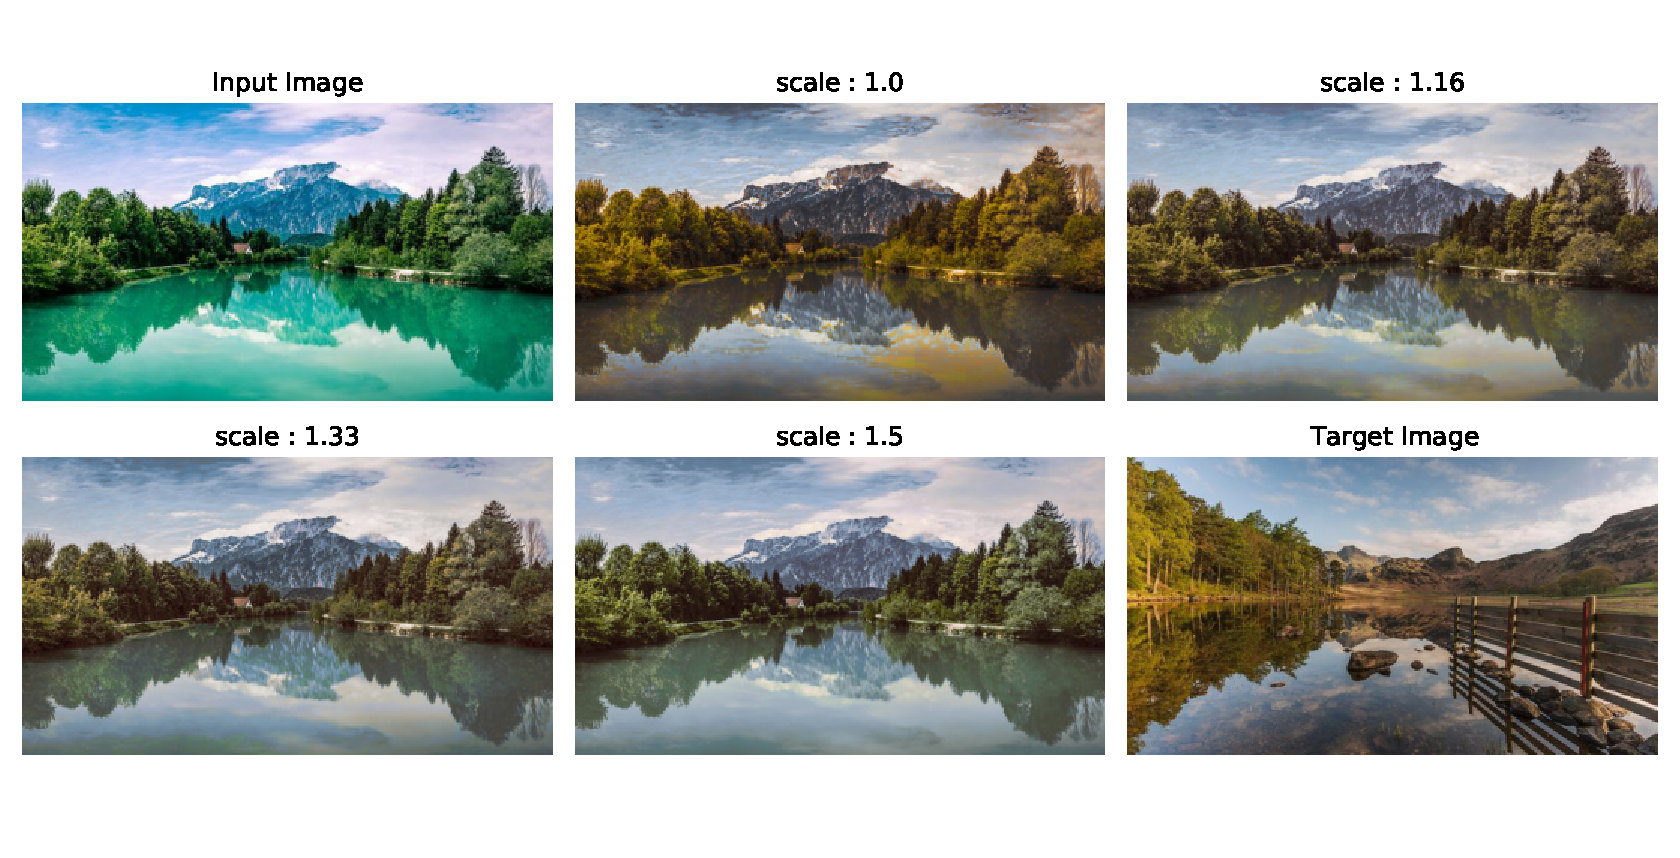
\includegraphics[width = \textwidth]{landscape12_6.pdf} \label{12_fig}
\caption{Color transfer for different upscaling values}
\end{figure}
\end{frame}

\subsection{Point Cloud Registration}

\begin{frame}
\frametitle{Results : Point Cloud Registration}



\begin{itemize}
\item Goal : Match a deformed subset of a point cloud to the original one, and find the transformation.
\item Method : Fast Iterative Sliced Transport, a variation of {\color{red}Iterative Closest Point}.
\end{itemize}

\begin{algorithm}[H]
\caption{Fast Iterative Closest Point}\label{FIST}
\scriptsize
%\begin{multicols}{2}
\hspace*{\algorithmicindent} \textbf{Input:} sorted $X,Y$\\
\hspace*{\algorithmicindent} \textbf{Output:} $X^*$ 
\begin{algorithmic}[2]
\State Initialize $X_0=X$
\For{$k$ from $0$ to $n_{iter}-1$}
	\State Choose $\omega$ random direction
	\State Compute the optimal Partial assignment $a$ between $Proj_\omega(X_k)$ and $Proj_\omega(Y)$
	\State Find the best transformation $T$ that transforms $X_k$ into $Y \circ a$ inside the set of allowed transformations
	\State Update $X_{k+1} \gets T(X_k)$
\EndFor
\State \Return{$X_{n_{iter}}$}
\end{algorithmic}
%\end{multicols}
\end{algorithm}

\end{frame}

%\begin{frame}
%\begin{figure}[H]
%\centering
%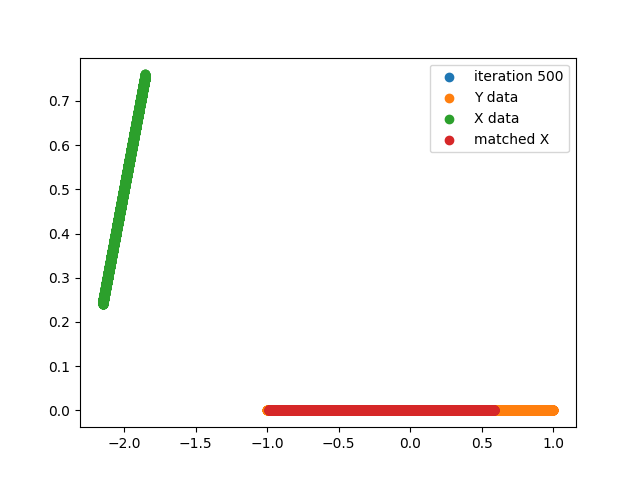
\includegraphics[width=0.9\textwidth, trim = 0cm 1cm 0cm 0cm]{line_shape.png}
%\caption{Point cloud Registration, $n=10000$, $m=8000$}\label{line_shape}
%\end{figure}
%\end{frame}

\begin{frame}
\begin{figure}[H]
\centering
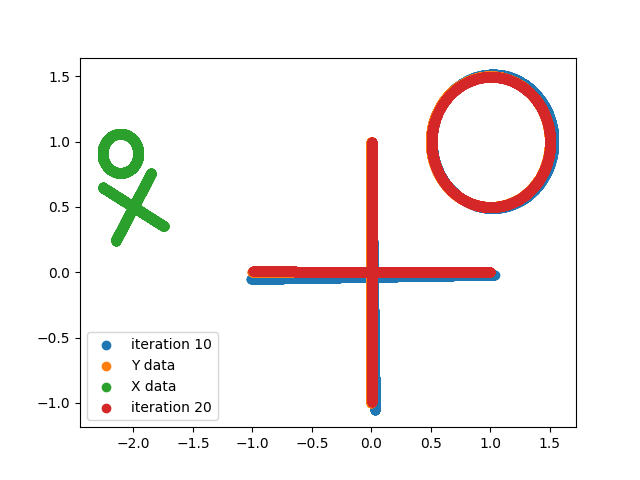
\includegraphics[width=0.49\textwidth, trim = 0cm 1cm 0cm 0cm]{circle_cross_shape.png}
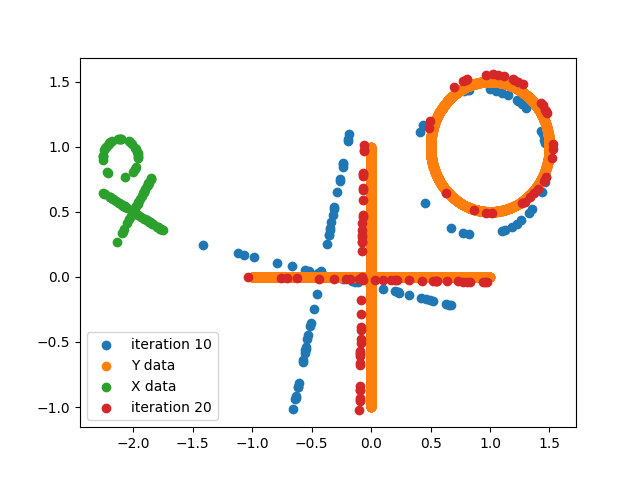
\includegraphics[width=0.49\textwidth, trim = 0cm 1cm 0cm 0cm]{circle_cross_shape2.png}
\caption{Point cloud Registration, $n=10000$, $m_1=8000$, $m_1=100$}\label{cc_shape}
\end{figure}
\end{frame}

\begin{frame}
\begin{figure}[H]
\centering
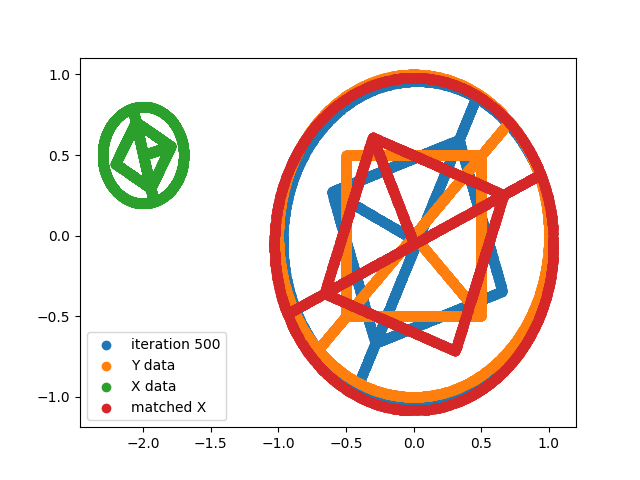
\includegraphics[width=0.49\textwidth, trim = 0cm 1cm 0cm 0cm]{circle_shape.png}
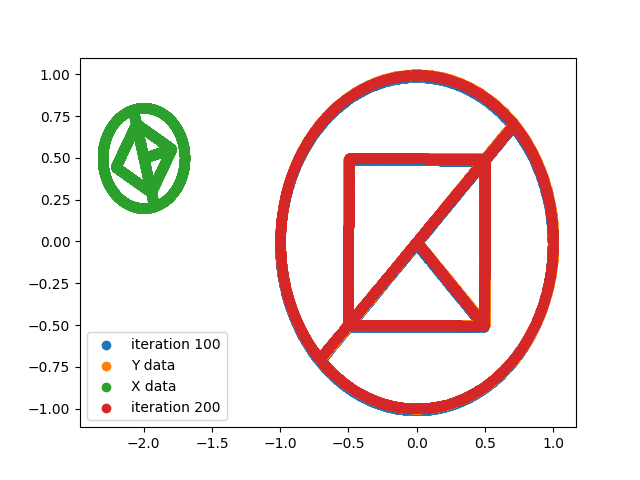
\includegraphics[width=0.49\textwidth, trim = 0cm 1cm 0cm 0cm]{circle_shape2.png}
\caption{Point cloud Registration, $n=10000$, $m=8000$}\label{cc_shape}
\end{figure}
\end{frame}

\section*{Conclusion}

\begin{frame}
\frametitle{Conclusion}
In this project I have :
\begin{itemize}
\item Made a {\color{red}fast python implementation of Sliced Partial Optimal Transport}. This method is fast and efficient in time and memory. 
\item Implemented a {\color{red}color transfer method} that works with images that have content with different proportions.
\item Implemented the {\color{red}FIST algorithm} for point cloud registration, which avoid the zero convergence problem.
\end{itemize}
\end{frame}

\begin{frame}
Thank you for your attention !
\end{frame}

\end{document}
